\hypertarget{kdbplugin_8hpp}{\section{kdbplugin.\+hpp File Reference}
\label{kdbplugin_8hpp}\index{kdbplugin.\+hpp@{kdbplugin.\+hpp}}
}


Helpers for creating plugins.  


{\ttfamily \#include $<$kdbplugin.\+h$>$}\\*
{\ttfamily \#include $<$key.\+hpp$>$}\\*
{\ttfamily \#include $<$keyset.\+hpp$>$}\\*
Include dependency graph for kdbplugin.\+hpp\+:
\nopagebreak
\begin{figure}[H]
\begin{center}
\leavevmode
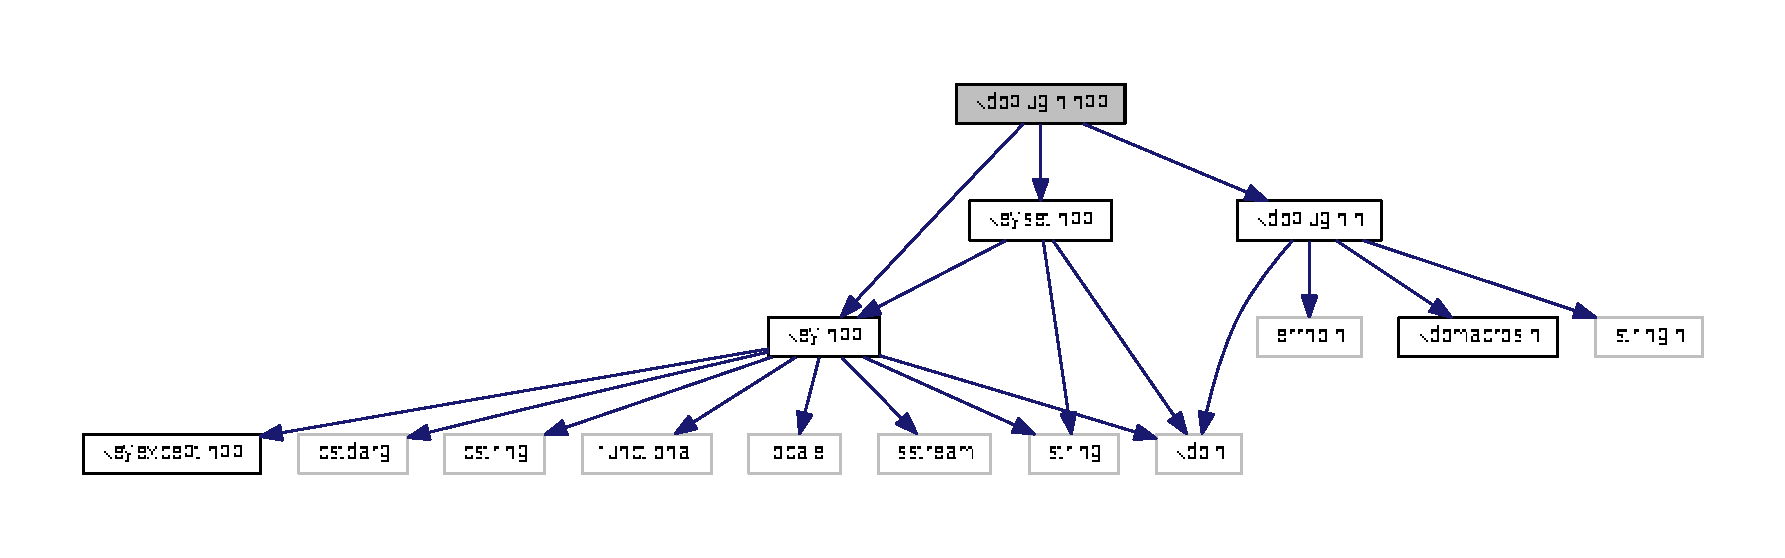
\includegraphics[width=350pt]{kdbplugin_8hpp__incl}
\end{center}
\end{figure}


\subsection{Detailed Description}
Helpers for creating plugins. 

Make sure to include kdberrors.\+h before including this file if you want warnings/errors to be added.

Proper usage\+: 
\begin{DoxyCode}
\textcolor{keyword}{using namespace }\hyperlink{namespaceckdb}{ckdb};
\textcolor{preprocessor}{#include <kdberrors.h>}
\textcolor{preprocessor}{#include <\hyperlink{kdbplugin_8hpp}{kdbplugin.hpp}>}

\textcolor{keyword}{typedef} Delegator<elektra::YourPluginClass> YPC;
\textcolor{comment}{// then e.g. YPC::open(handle, errorKey);}
\end{DoxyCode}


\begin{DoxyCopyright}{Copyright}
B\+S\+D License (see doc/\+L\+I\+C\+E\+N\+S\+E.\+md or \href{http://www.libelektra.org}{\tt http\+://www.\+libelektra.\+org}) 
\end{DoxyCopyright}
